\documentclass{standalone}
\usepackage{tikz}
\usetikzlibrary{patterns, positioning}


\begin{document}
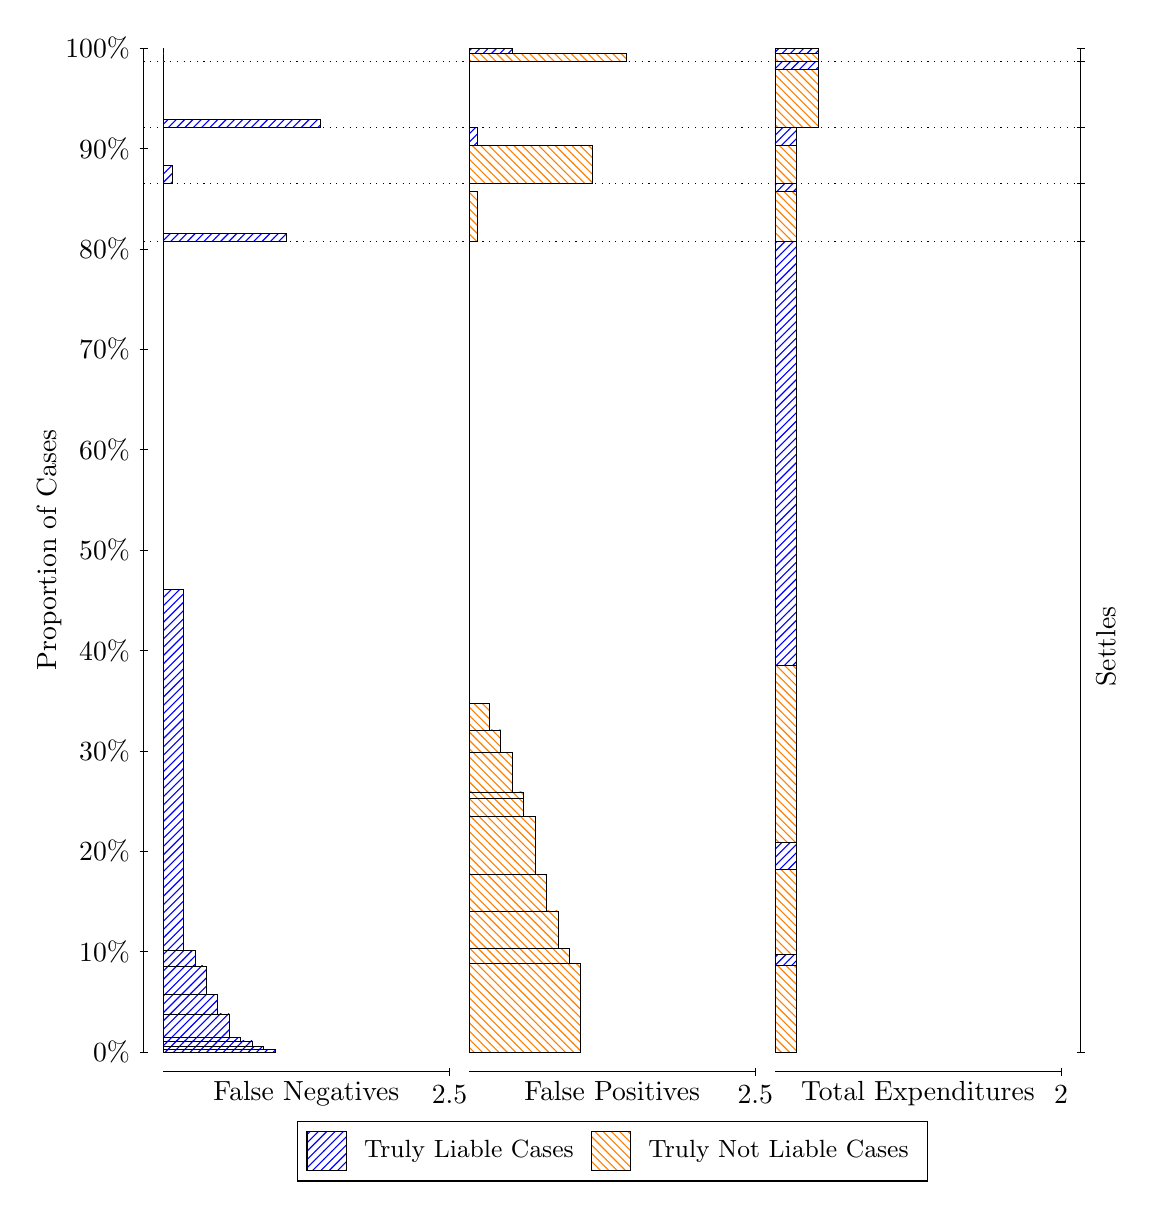
\begin{tikzpicture}
\draw[black, very thin] (1.5,1.75) -- (1.5,14.5);
\node[rotate=90, text=black, anchor=center] at (0.3, 8.125) {Proportion of Cases};
\draw[black, very thin] (1.45,1.75) -- (1.55,1.75);
\node[text=black, anchor=east] at (1.45, 1.75) {0\%};
\draw[black, very thin] (1.45,3.025) -- (1.55,3.025);
\node[text=black, anchor=east] at (1.45, 3.025) {10\%};
\draw[black, very thin] (1.45,4.3) -- (1.55,4.3);
\node[text=black, anchor=east] at (1.45, 4.3) {20\%};
\draw[black, very thin] (1.45,5.575) -- (1.55,5.575);
\node[text=black, anchor=east] at (1.45, 5.575) {30\%};
\draw[black, very thin] (1.45,6.85) -- (1.55,6.85);
\node[text=black, anchor=east] at (1.45, 6.85) {40\%};
\draw[black, very thin] (1.45,8.125) -- (1.55,8.125);
\node[text=black, anchor=east] at (1.45, 8.125) {50\%};
\draw[black, very thin] (1.45,9.4) -- (1.55,9.4);
\node[text=black, anchor=east] at (1.45, 9.4) {60\%};
\draw[black, very thin] (1.45,10.675) -- (1.55,10.675);
\node[text=black, anchor=east] at (1.45, 10.675) {70\%};
\draw[black, very thin] (1.45,11.95) -- (1.55,11.95);
\node[text=black, anchor=east] at (1.45, 11.95) {80\%};
\draw[black, very thin] (1.45,13.225) -- (1.55,13.225);
\node[text=black, anchor=east] at (1.45, 13.225) {90\%};
\draw[black, very thin] (1.45,14.5) -- (1.55,14.5);
\node[text=black, anchor=east] at (1.45, 14.5) {100\%};

\draw[black, very thin] (13.4,1.75) -- (13.4,14.5);
\draw[black, very thin] (13.35,1.75) -- (13.45,1.75);
\node[anchor=west] at (13.35, 1.75) {};
\draw[black, very thin] (13.35,12.047) -- (13.45,12.047);
\node[anchor=west] at (13.35, 12.047) {};
\draw[black, very thin] (13.35,12.781) -- (13.45,12.781);
\node[anchor=west] at (13.35, 12.781) {};
\draw[black, very thin] (13.35,13.492) -- (13.45,13.492);
\node[anchor=west] at (13.35, 13.492) {};
\draw[black, very thin] (13.35,14.332) -- (13.45,14.332);
\node[anchor=west] at (13.35, 14.332) {};
\draw[black, very thin] (13.35,14.5) -- (13.45,14.5);
\node[anchor=west] at (13.35, 14.5) {};

\draw[black, very thin, pattern color=blue, pattern=north east lines] (1.75,1.75) rectangle (3.167,1.7868);
\draw[black, very thin, pattern color=blue, pattern=north east lines] (1.75,1.7868) rectangle (3.0217,1.8229);
\draw[black, very thin, pattern color=blue, pattern=north east lines] (1.75,1.8229) rectangle (2.8763,1.89);
\draw[black, very thin, pattern color=blue, pattern=north east lines] (1.75,1.89) rectangle (2.731,1.9355);
\draw[black, very thin, pattern color=blue, pattern=north east lines] (1.75,1.9355) rectangle (2.5857,2.2334);
\draw[black, very thin, pattern color=blue, pattern=north east lines] (1.75,2.2334) rectangle (2.4403,2.4777);
\draw[black, very thin, pattern color=blue, pattern=north east lines] (1.75,2.4777) rectangle (2.295,2.844);
\draw[black, very thin, pattern color=blue, pattern=north east lines] (1.75,2.844) rectangle (2.1497,3.0415);
\draw[black, very thin, pattern color=blue, pattern=north east lines] (1.75,3.0415) rectangle (2.0043,7.6207);
\draw[black, very thin, pattern color=orange, pattern=north west lines] (1.75,7.6207) rectangle (1.75,12.047);
\draw[black, very thin, pattern color=blue, pattern=north east lines] (1.75,12.047) rectangle (3.3123,12.147);
\draw[black, very thin, pattern color=orange, pattern=north west lines] (1.75,12.147) rectangle (1.75,12.781);
\draw[black, very thin, pattern color=blue, pattern=north east lines] (1.75,12.781) rectangle (1.859,13.013);
\draw[black, very thin, pattern color=orange, pattern=north west lines] (1.75,13.013) rectangle (1.75,13.492);
\draw[black, very thin, pattern color=blue, pattern=north east lines] (1.75,13.492) rectangle (3.7483,13.594);
\draw[black, very thin, pattern color=orange, pattern=north west lines] (1.75,13.594) rectangle (1.75,14.332);
\draw[black, very thin, pattern color=orange, pattern=north west lines] (1.75,14.332) rectangle (1.75,14.43);
\draw[black, very thin, pattern color=blue, pattern=north east lines] (1.75,14.43) rectangle (1.75,14.5);
\draw[black, very thin, pattern color=orange, pattern=north west lines] (5.6333,1.75) rectangle (7.0503,2.8718);
\draw[black, very thin, pattern color=orange, pattern=north west lines] (5.6333,2.8718) rectangle (6.905,3.0675);
\draw[black, very thin, pattern color=orange, pattern=north west lines] (5.6333,3.0675) rectangle (6.7597,3.5424);
\draw[black, very thin, pattern color=orange, pattern=north west lines] (5.6333,3.5424) rectangle (6.6143,4.0016);
\draw[black, very thin, pattern color=orange, pattern=north west lines] (5.6333,4.0016) rectangle (6.469,4.7447);
\draw[black, very thin, pattern color=orange, pattern=north west lines] (5.6333,4.7447) rectangle (6.3237,4.9693);
\draw[black, very thin, pattern color=orange, pattern=north west lines] (5.6333,4.9693) rectangle (6.3237,5.053);
\draw[black, very thin, pattern color=orange, pattern=north west lines] (5.6333,5.053) rectangle (6.1783,5.5572);
\draw[black, very thin, pattern color=orange, pattern=north west lines] (5.6333,5.5572) rectangle (6.033,5.8401);
\draw[black, very thin, pattern color=orange, pattern=north west lines] (5.6333,5.8401) rectangle (5.8877,6.176);
\draw[black, very thin, pattern color=blue, pattern=north east lines] (5.6333,6.176) rectangle (5.6333,12.047);
\draw[black, very thin, pattern color=orange, pattern=north west lines] (5.6333,12.047) rectangle (5.7423,12.68);
\draw[black, very thin, pattern color=blue, pattern=north east lines] (5.6333,12.68) rectangle (5.6333,12.781);
\draw[black, very thin, pattern color=orange, pattern=north west lines] (5.6333,12.781) rectangle (7.1957,13.26);
\draw[black, very thin, pattern color=blue, pattern=north east lines] (5.6333,13.26) rectangle (5.7423,13.492);
\draw[black, very thin, pattern color=orange, pattern=north west lines] (5.6333,13.492) rectangle (5.6333,14.231);
\draw[black, very thin, pattern color=blue, pattern=north east lines] (5.6333,14.231) rectangle (5.6333,14.332);
\draw[black, very thin, pattern color=orange, pattern=north west lines] (5.6333,14.332) rectangle (7.6317,14.43);
\draw[black, very thin, pattern color=blue, pattern=north east lines] (5.6333,14.43) rectangle (6.1783,14.5);
\draw[black, very thin, pattern color=orange, pattern=north west lines] (9.5167,1.75) rectangle (9.7892,2.8454);
\draw[black, very thin, pattern color=blue, pattern=north east lines] (9.5167,2.8454) rectangle (9.7892,2.994);
\draw[black, very thin, pattern color=orange, pattern=north west lines] (9.5167,2.994) rectangle (9.7892,4.073);
\draw[black, very thin, pattern color=blue, pattern=north east lines] (9.5167,4.073) rectangle (9.7892,4.4078);
\draw[black, very thin, pattern color=orange, pattern=north west lines] (9.5167,4.4078) rectangle (9.7892,6.6594);
\draw[black, very thin, pattern color=blue, pattern=north east lines] (9.5167,6.6594) rectangle (9.7892,12.047);
\draw[black, very thin, pattern color=orange, pattern=north west lines] (9.5167,12.047) rectangle (9.7892,12.68);
\draw[black, very thin, pattern color=blue, pattern=north east lines] (9.5167,12.68) rectangle (9.7892,12.781);
\draw[black, very thin, pattern color=orange, pattern=north west lines] (9.5167,12.781) rectangle (9.7892,13.26);
\draw[black, very thin, pattern color=blue, pattern=north east lines] (9.5167,13.26) rectangle (9.7892,13.492);
\draw[black, very thin, pattern color=orange, pattern=north west lines] (9.5167,13.492) rectangle (10.062,14.231);
\draw[black, very thin, pattern color=blue, pattern=north east lines] (9.5167,14.231) rectangle (10.062,14.332);
\draw[black, very thin, pattern color=orange, pattern=north west lines] (9.5167,14.332) rectangle (10.062,14.43);
\draw[black, very thin, pattern color=blue, pattern=north east lines] (9.5167,14.43) rectangle (10.062,14.5);
\draw[black, dotted] (1.5,12.047) -- (13.4,12.047);
\draw[black, dotted] (1.5,12.781) -- (13.4,12.781);
\draw[black, dotted] (1.5,13.492) -- (13.4,13.492);
\draw[black, dotted] (1.5,14.332) -- (13.4,14.332);
\draw[black, very thin] (1.75,1.5) -- (5.3833,1.5);
\node[text=black, anchor=north] at (3.5667, 1.5) {False Negatives};
\draw[black, very thin] (5.3833,1.45) -- (5.3833,1.55);
\node[text=black, anchor=north] at (5.3833, 1.45) {2.5};

\draw[black, very thin] (5.6333,1.5) -- (9.2667,1.5);
\node[text=black, anchor=north] at (7.45, 1.5) {False Positives};
\draw[black, very thin] (9.2667,1.45) -- (9.2667,1.55);
\node[text=black, anchor=north] at (9.2667, 1.45) {2.5};

\draw[black, very thin] (9.5167,1.5) -- (13.15,1.5);
\node[text=black, anchor=north] at (11.333, 1.5) {Total Expenditures};
\draw[black, very thin] (13.15,1.45) -- (13.15,1.55);
\node[text=black, anchor=north] at (13.15, 1.45) {2};

\node[text=black, centered, rotate=90] at (13.72, 6.8984) {Settles};





\draw (7.449999999999999,1.5) node[draw=none] (baseCoordinate) {};
\begin{scope}[align=center]
        \matrix[scale=0.5, draw=black, below=0.5cm of baseCoordinate, nodes={draw}, column sep=0.1cm]{
            \node[rectangle, draw, minimum width=0.5cm, minimum height=0.5cm, pattern color=blue, pattern=north east lines] {}; &
            \node[draw=none, font=\small, text=black] (B) {Truly Liable Cases}; &
            \node[rectangle, draw, minimum width=0.5cm, minimum height=0.5cm, pattern color=orange, pattern=north west lines] {}; &
            \node[draw=none, font=\small, text=black] (B) {Truly Not Liable Cases}; \\
            };
\end{scope}

\end{tikzpicture}
\end{document}